\clearpage
\section{\markg{Voice flow}}
\label{sec:voice_flow}
È resa disponibile all'utente una \markg{skill} utilizzabile con l'assistente \markg{Amazon} \markg{Alexa} che permette l'avvio dei \markg{workflow} presenti nell'applicazione tramite comandi vocali.
L'immagine sottostante rappresenta lo schema di un \markg{voice flow} generico avviato tramite la \markg{skill}.
\begin{figure}[H]
	\centering
	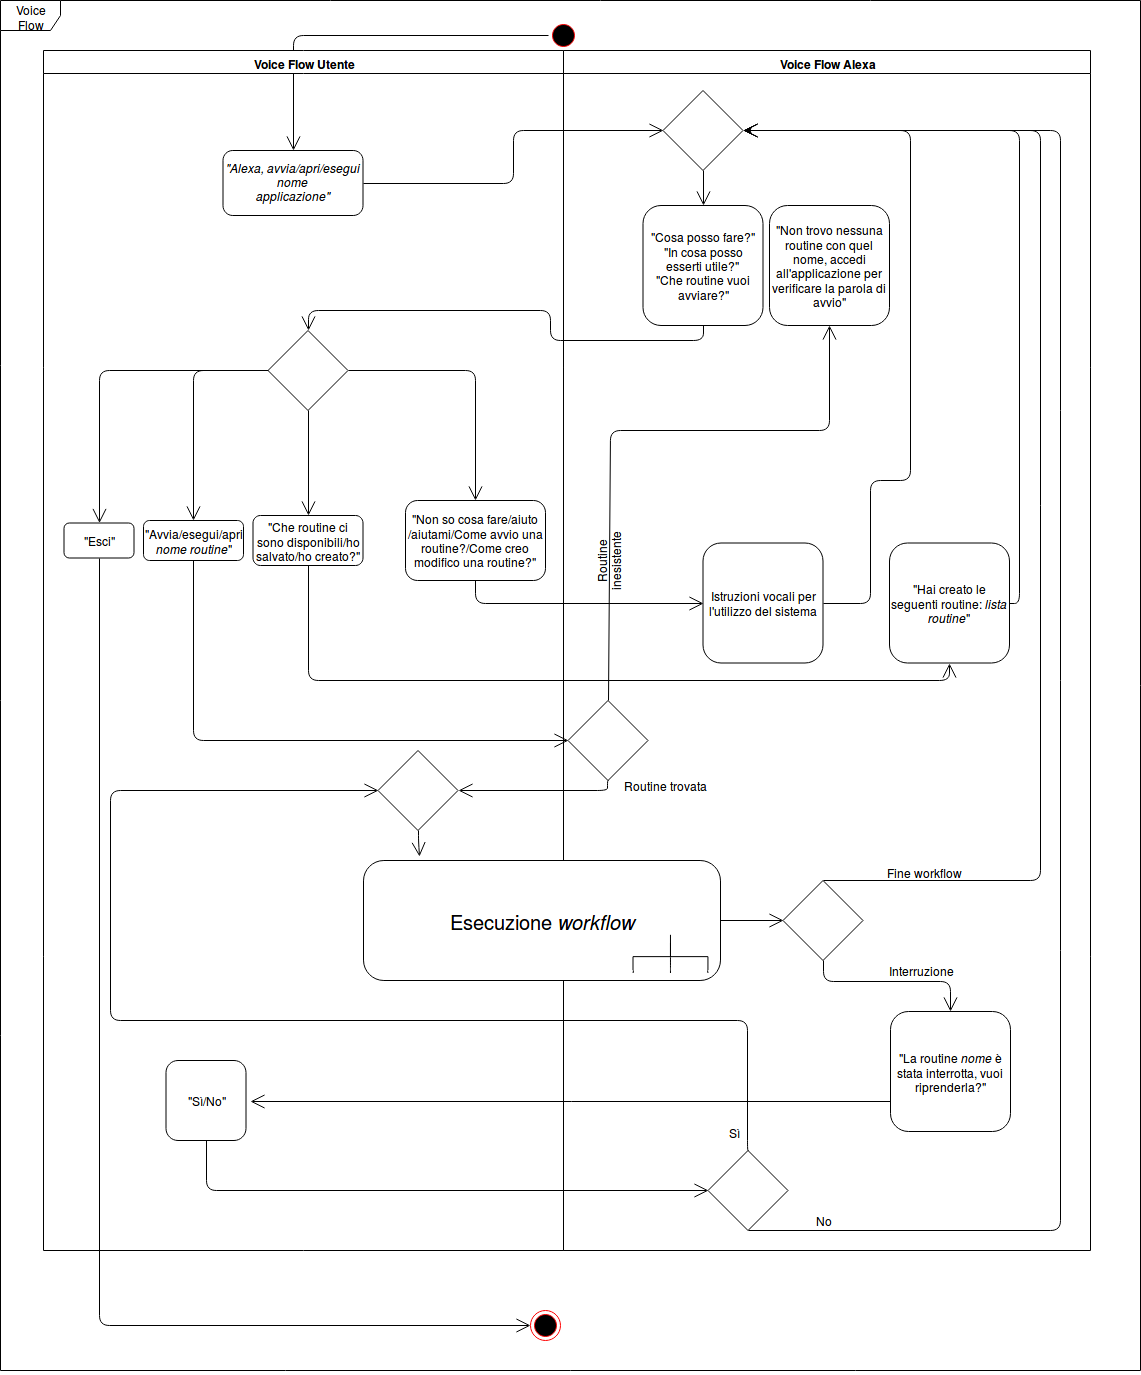
\includegraphics[width=15cm,keepaspectratio]{../includes/pics/voice_flow_alexa-utente_UML.png}
	\caption{\label{fig:mission}Schema \markg{voice flow} generico}
\end{figure}
\begin{figure}[H]
	\centering
	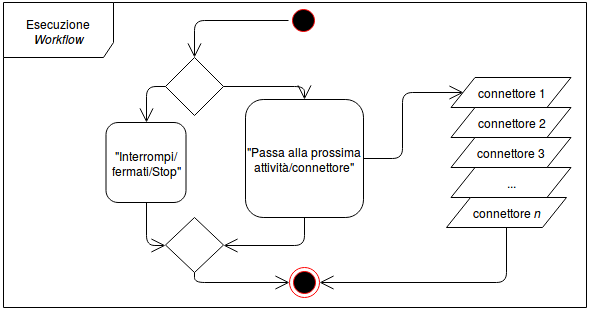
\includegraphics[width=15cm,keepaspectratio]{../includes/pics/voice_flow_alexa-utente_esecuzione_workflow.png}
	\caption{\label{fig:mission}Schema \markg{voice flow} generico}
\end{figure}
\subsection{Interazione vocale utente - Assistente vocale}
\label{sec:iterazione_vocale_utente}
Durante l'esecuzione del \markg{workflow} alcuni \markg{connettori} potrebbero necessitare di un'ulteriore interazione vocale tra l'utente e l'assistente vocale. Di seguito viene esplicato in che modo è strutturato il dialogo tra l'utente e \markg{Amazon} \markg{Alexa}.
\subsection{Interazioni UC21 - Connettore: imposta sveglia}
\label{sec:connettore_sveglia}
\begin{itemize}
        \item \markg{Alexa}: "Vuoi/Desideri impostare una sveglia?".
        \item Utente: "Sì/No/{\it orario}".
        \begin{itemize}
         \item{Risposta {\it "Sì"} }, \markg{Alexa}:"Che orario vuoi impostare per la sveglia?".
         \begin{itemize}
              \item{Risposta {\it orario} corretto}, \markg{Alexa}:"La sveglia è stata impostata alle ore {\it orario}".
              \item{Risposta {\it orario} errato}, \markg{Alexa}:  {\it UC21.2 - Ricezione notifica orario errato}
         \end{itemize}
         \item{Risposta {\it "No"} }, il sistema passa al \markg{connettore} successivo o termina il \markg{workflow} se non sono presenti altri \markg{connettori}.
         \item{Risposta {\it orario} corretto}, \markg{Alexa}:"La sveglia è stata impostata alle ore {\it orario}".
         \item{Risposta {\it orario} errato}, \markg{Alexa}:  {\it UC21.2 - Ricezione notifica orario errato}
         \end{itemize}
    \end{itemize}

\subsection{Interazioni UC22 - Connettore: riproduzione musica}
\label{sec:connettore_musica}
 \begin{itemize}
        \item \markg{Alexa}: "Cosa/chi vuoi ascoltare?".
        \item Utente: "{\it nome artista}/{\it nome traccia}".
        \begin{itemize}
         \item{Risposta {\it nome artista} corretto}, il sistema fa riprodurre ad \markg{Alexa} le tracce dell'artista.
        \item{Risposta {\it nome artista} errato}, \markg{Alexa}:  {\it UC22.1 - Ricezione notifica titolo o artista non riconosciuto}.
        \item{Risposta {\it nome traccia} corretto}, il sistema fa riprodurre ad \markg{Alexa} la traccia.
        \item{Risposta {\it nome traccia} errato}, \markg{Alexa}:  {\it UC22.1 - Ricezione notifica titolo o artista non riconosciuto}.
         \end{itemize}
    \end{itemize}


\subsection{Interazioni UC24 - Connettore: lettura calendario}
\label{sec:connettore_lettura_calendario}
\begin{itemize}
        \item \markg{Alexa}: "Domani hai fissato i seguenti eventi: {\it lista eventi}, vuoi sapere gli eventi del resto della settimana?".
        \item Utente: "Sì/No".
        \begin{itemize}
         \item{Risposta "Sì"}, \markg{Alexa}: "Hai fissato i seguenti eventi: {\it lista eventi successivi}".
         \item{Risposta "No"}, il sistema passa al \markg{connettore} successivo o termina il \markg{workflow} se non sono presenti altri \markg{connettori}.
         \end{itemize}
    \end{itemize}


\subsection{Interazioni UC25 - Connettore: aggiunta evento calendario}
\label{sec:connettore_evento_calendario}
 \begin{itemize}
        \item \markg{Alexa}: "Vuoi aggiungere un evento?".
        \item Utente: "Sì/No".
        \begin{itemize}
         \item{Risposta "Sì"}, \markg{Alexa}: "In che data?".
         \item Utente: "{\it data}".
         \begin{itemize}
             \item{Risposta {\it data in formato corretto}}, \markg{Alexa}: "Che nome vuoi dare all'evento?".
             \item Utente: {\it nome evento}.
             \item \markg{Alexa}: "Ho creato l'evento {\it nome evento} in data {\it data}."
            \item{Risposta "{\it data in formato non corretto}}, \markg{Alexa}: {\it UC25.1 - Ricezione notifica data errata}.
         \end{itemize}
         \item{Risposta "No"}, il sistema passa al \markg{connettore} successivo o termina il \markg{workflow} se non sono presenti altri \markg{connettori}.
         \end{itemize}
    \end{itemize}

\subsection{Interazioni UC26 - Connettore: scrittura nota}
\label{sec:connettore_nota}
\begin{itemize}
        \item \markg{Alexa}: "Vuoi aggiungere una nota?".
        \item Utente: "Sì/No".
        \begin{itemize}
         \item{Risposta "Sì"}, \markg{Alexa}: "Dimmi pure/Che nota aggiungo?".
         \item Utente: "{\it Corpo nota}".
         \item{Risposta "No"}, il sistema passa al \markg{connettore} successivo o termina il \markg{workflow} se non sono presenti altri \markg{connettori}.
         \end{itemize}
    \end{itemize}


\subsection{Interazioni UC27 - Connettore: pubblicazione e lettura Tweet}
\label{sec:connettore_twitter}
 \begin{itemize}
        \item \markg{Alexa}: "Cosa vuoi fare? Puoi: pubblicare un tweet, leggere i tweet di {\it Account impostato da \markg{connettore}}, leggere i tweet della tua bacheca".
        \item Utente: "Voglio pubblicare un tweet/Voglio leggere i tweet di {\it Account impostato da \markg{connettore}}/Voglio leggere i tweet della mia bacheca".
        \begin{itemize}
         \item{Risposta "Voglio pubblicare un tweet"}, \markg{Alexa}: "{\it UC27.1 - Pubblicazione tweet}".
         \item{Risposta "Voglio leggere i tweet di {\it Account impostato da \markg{connettore}}"}, \markg{Alexa}: "{\it UC27.2 - Lettura ultimi tweet da singolo account}".
         \item{Risposta "Voglio leggere i tweet della mia bacheca"}, \markg{Alexa}: "{\it UC27.3 - Lettura tweet bacheca personale}".
         \end{itemize}
    \end{itemize}


\subsection{Interazioni UC27.1 - Pubblicazione tweet}
\label{sec:connettore_twitter_scrittura}
\begin{itemize}
        \item \markg{Alexa}: "Dimmi pure cosa vuoi pubblicare./Cosa vuoi rispondere?".
        \item Utente: "{\it corpo tweet}".
        \begin{itemize}
        \item \markg{Alexa}: "Ho pubblicato il tuo tweet".
           \end{itemize}
        \item Utene: "{\it corpo tweet con più di 280 caratteri}".
           \begin{itemize}
        \item \markg{Alexa}: "{\it UC27.1.1 - Ricezione notifica fine caratteri disponibili}".
           \end{itemize}
        
    \end{itemize}


\subsection{Interazioni UC27.2 - Lettura ultimi tweet da singolo account}
\label{sec:connettore_twitter_profilo}
 \begin{itemize}
        \item \markg{Alexa}: "Gli ultimi tweet di {\it Account impostato da \markg{connettore}} sono {\it lettura corpo tweet}".
        \item Utente che interrompe dopo l'ascolto di un tweet: "Voglio rispondere".
        \item \markg{Alexa}: "{\it UC27.1 - Pubblicazione tweet}".
    \end{itemize}


\subsection{Interazioni UC27.3 - Connettore: lettura tweet bacheca personale}
\label{sec:connettore_twitter_bacheca}
 \begin{itemize}
        \item \markg{Alexa}: "Nella tua bacheca ho trovato i seguenti tweet: {\it lettura corpo tweet}".
        \item Utente che interrompe dopo l'ascolto di un tweet: "Voglio rispondere".
        \item \markg{Alexa}: "{\it UC27.1 - Pubblicazione tweet}".
    \end{itemize}


\subsection{Interazioni  UC28 - Connettore: operazioni con \markg{Trello}}
\label{sec:connettore_trello} 
 \begin{itemize}
        \item \markg{Alexa}: "Cosa desideri fare nella bacheca {\it bacheca impostata}? Puoi: leggere le tue schede, aggiungere una nuova scheda, spostare una scheda tra liste".
        \item Utente: "Voglio leggere le mie schede/Voglio aggiungere una scheda/Voglio spostare una scheda.".
        \begin{itemize}
         \item{Risposta "Voglio leggere le mie schede"}, \markg{Alexa}: "{\it UC28.1 - Lettura lista da bacheca \markg{Trello}}".
         \item{Risposta "Voglio aggiungere una scheda"}, \markg{Alexa}: "{\it  UC28.2 - Creazione scheda in bacheca \markg{Trello}}".
         \item{Risposta "Voglio spostare una scheda"}, \markg{Alexa}: "{\it UC28.3 - Spostamento scheda tra liste \markg{Trello}}".
         \end{itemize}
    \end{itemize}


\subsection{Interazioni UC28.1 - Lettura lista da bacheca \markg{Trello}}
\label{sec:connettore_trello_leggi_bacheca}
 \begin{itemize}
        \item \markg{Alexa}: "Che lista devo leggere?".
        \item Utente: "{\it nome lista esistente}".
        \begin{itemize}
        \item \markg{Alexa}: "{\it lettura lista}".
           \end{itemize}
        \item Utene: "{\it nome lista inesistente}".
           \begin{itemize}
        \item \markg{Alexa}: "{\it UC28.6 - Ricezione notifica lista inesistente}".
           \end{itemize}
    \end{itemize}


\subsection{Interazioni UC28.2 - Creazione scheda in bacheca \markg{Trello}}
\label{sec:connettore_trello_crea_bacheca}
 \begin{itemize}
        \item \markg{Alexa}: "In che lista vuoi che aggiunga la scheda?".
        \item Utente: "{\it nome lista esistente}".
        \begin{itemize}
        \item \markg{Alexa}: "Dimmi pure".
        \item Utente: "{\it corpo scheda}".
           \end{itemize}
        \item Utente: "{\it nome lista inesistente}".
           \begin{itemize}
        \item \markg{Alexa}: "{\it UC28.6 - Ricezione notifica lista inesistente}".
           \end{itemize}
    \end{itemize}


\subsection{Interazioni  UC28.3 - Spostamento scheda tra liste \markg{Trello}}
\label{sec:connettore_trello_sposta_scheda}
 \begin{itemize}
        \item \markg{Alexa}: "Da che lista vuoi spostare la scheda?".
        \item Utente: "{\it nome lista esistente}".
        \begin{itemize}
        \item \markg{Alexa}: "Che scheda vuoi spostare".
       
        \item Utente: "{\it nome scheda esistente}".
        \begin{itemize}
        \item \markg{Alexa}: "In che lista vuoi spostare la scheda?"
          \item Utente: "{\it nome lista esistente}".
          \begin{itemize}
              \item \markg{Alexa}: "Scheda spostata con successo".
          \end{itemize}
           \item Utente: "{\it nome lista inesistente}".
           \begin{itemize}
        \item \markg{Alexa}: "{\it UC28.6 - Ricezione notifica lista inesistente}".
        \end{itemize}
      \end{itemize}
      
     \item Utente: "{\it nome scheda inesistente}".
     \begin{itemize}
           \item \markg{Alexa}: "{\it UC28.3.1 - Ricezione notifica scheda inesistente}".
           \end{itemize}
            \end{itemize}
        \item Utente: "{\it nome lista inesistente}".
           \begin{itemize}
        \item \markg{Alexa}: "{\it UC28.6 - Ricezione notifica lista inesistente}".
           \end{itemize}
    \end{itemize}
